% OpenStreetMap pour Toulibre
%
% Author: Eric Marsden <eric.marsden@free.fr>
% Time-stamp: <2009-11-08 emarsden>



\documentclass[slidestop,serif,10pt]{beamer}
\usepackage[utf8x]{inputenc}
\usepackage[T1]{fontenc}
\usepackage[francais]{babel}
\usepackage{lmodern}
\usepackage{pifont}
\usepackage{wasysym}
\usepackage{yfonts}
\usepackage{euscript}
\usepackage{eufrak}
\usepackage{marvosym}
\usepackage{mdwlist}
\usepackage{sverb}
\usepackage{fancybox}
\usepackage{tabularx}
\usepackage{graphicx}
\usepackage{movie15}
\usepackage{lettrine}
\usepackage{verbatim}
\usepackage{microtype}


%% palatino default:
% \renewcommand{\rmdefault}{ppl}
% \renewcommand{\sfdefault}{phv}

%% Charter default:
\renewcommand{\rmdefault}{bch}
\renewcommand{\bfdefault}{b}


%% misc symbols
%% \Pointinghand
%% \checked
%% \lightning
%% \frownie, \smilie
%% `` = \ding{125}
%% '' = \ding{126}


\usepackage{beamerthemeemarsden}


\beamerboxesdeclarecolorscheme{alert}{red}{red!15!bg}

% beamer versions
% \makeatletter
% \newenvironment{ecmslide}{}{}
% \def\beginecmslide\frame
% \def\endecmslide{}
% \makeatother
\newcommand{\heading}[1]{\frametitle{\fontfamily{ppl}\selectfont #1}}
\newcommand{\ecmfrownie}{\raisebox{-0.5ex}{\color{orange}\Huge \frownie}}
\newcommand{\ecmsmiley}{\raisebox{-0.5ex}{\color{orange}\Huge \smiley}}


\newcommand{\ecmfontcharter}{\fontfamily{ppl}\selectfont}
\newcommand{\ecmfontpalatino}{\fontfamily{bch}\selectfont}
\newcommand{\ecmfontpag}{\fontfamily{pag}\selectfont}

\newcommand{\ecmsetupplan}{
  \sffamily\ecmfontpag\Large
  \setlength{\baselineskip}{1.4\baselineskip}
  \hypersetup{pdfpagetransition=Dissolve}
  % \hypersetup{pdfpagetransition=Blinds}
  % \hypersetup{pdfpagetransition=Wipe}
  \vspace{1cm}
}


\setlength{\parskip}{0.2\baselineskip}
\setlength{\parindent}{0mm}
\setlength{\parsep}{0mm}
\hyphenpenalty 10000
\raggedright

% \renewcommand{\labelitemi}{\textbullet}
% \renewcommand{\labelitemii}{\tiny$\diamondsuit$}
% \newcommand{\whatis}[1]
%   {\renewcommand{\labelitemi}{$\blacktriangleright$}%
%    \renewcommand{\labelitemii}{$\blacktriangleright$}%
%    \begin{itemize} %
%    \item #1
%    \end{itemize}
%    \renewcommand{\labelitemi}{\textbullet}
%    \renewcommand{\labelitemii}{\tiny $\diamondsuit$}}

\def\labelitemi\textbullet


\title{Le projet OpenStreetMap}
\author{Éric Marsden}
\date{Juin 2009}
% \titlegraphic{\includegraphics[width=3cm]{common-figures/LAAS}}

\hypersetup{
   pdftitle={Le projet OpenStreetMap},
   pdfauthor={Eric Marsden},
   pdfkeywords={openstreetmap, mapping, cartographie},
   pdftoolbar=false,
   % pdfmenubar=false,
   pdfpagemode={FullScreen}
}


\definecolor{gray}{rgb}{0.2,0.2,0.2}
\definecolor{purple}{rgb}{0.6,0.35,0.6}
\definecolor{orange}{rgb}{1,0.7734375,0.1171875}
\definecolor{darkyellow}{rgb}{0.8,0.8,0.2}
\definecolor{darkgreen}{rgb}{0.29296875,0.46484375,0.35546875}



\def\listingsize{\footnotesize}
\setlength\listingindent{0cm}

\begin{document}



%% FIXME don't number this first slide
\frame[plain]
{
  \vspace{1cm}
  \begin{center}

%     {\color{structure} \fontfamily{ppl}\selectfont \Huge \em
%       Le projet \\[0.4cm]
%       OpenStreetMap \\[0.5cm]}
    
\includegraphics[width=0.9\textwidth]{figures/logo-OSM}

    \small 
    \vspace{1.1cm}
    Éric Marsden  \texttt{<eric.marsden@free.fr>}
    \vspace{1.2cm}

    Toulibre, juin 2009
  \end{center}
}

%% osm-intro.tex
%%


\section{Introduction}

\frame { \heading{OSM: kesako?} \vfill

  OpenStreetMap (OSM) est un \textbf{projet collaboratif} visant à créer des
  \textbf{cartes libres}

  \begin{itemize}
  \item données et cartes rediffusables sous licence libre 
\includegraphics[width=1.2cm]{figures/cc-by-sa}
  \item couvrant toute la planète
  \item modèle de contribution à la wiki: chacun peut ajouter des
    traces GPS, corriger le nom d'une rue
  \item projet fondé en 2004, croissance très rapide
  \end{itemize}

  \vfil
  
\begin{beamerboxesrounded}[width=\textwidth,scheme=alert,shadow=true]{} \sffamily\footnotesize
  «OpenStreetMap is a project aimed squarely at creating and
  providing free geographic data such as street maps to anyone who
  wants them. The project was started because most maps you think of
  as free actually have legal or technical restrictions on their use,
  holding back people from using them in creative, productive or
  unexpected ways.»
\end{beamerboxesrounded}

}


%% animation Toulouse timeline


% \frame{\includegraphics[width=0.95\textwidth]{figures/toulouse-map}}
% \frame{\includegraphics[width=0.95\textwidth]{figures/toulouse-zoom}}



\frame{
  %% http://www.flickr.com/photos/stevefaeembra/3674760067/sizes/o/in/set-72157620624558941/
 \hskip-0.5cm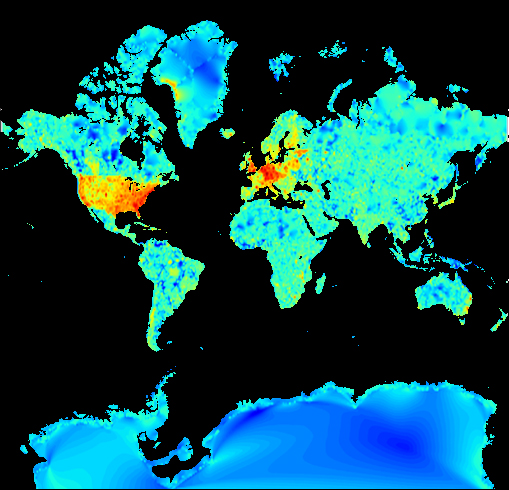
\includegraphics[width=0.8\textwidth]{figures/osm-heatmap}

 %% http://www.openstreetmap.org/stats/data_stats.html

\begin{tikzpicture}[remember picture,overlay,font={\footnotesize},text
    width=2cm,text centered]
   \node[starburst,fill=yellow,draw=red,line width=2pt,shift={(-2cm,-2cm)}]
      at (current page.north east) {190\,535 utilisateurs};
   \node[starburst,fill=yellow,draw=red,line width=2pt,shift={(-3cm,-7.1cm)}]
      at (current page.north east) {1\,300\,501\,165 points GPS};
\end{tikzpicture}
}




\frame{ \heading{Des données libres?} \vfill

  Libertés que devraient offrir des données géographiques:

  \begin{itemize}
  \item utiliser les données dans n'importe quel but
  \item étudier les données et de les adapter
  \item distribuer des copies
  \item modifier les données et rendre publiques ces modifications
  \end{itemize}

\begin{itemize}
% \item[{\color{red}\ding{56}}]
\item[\ecmfrownie] Les principales sources de données aujourd'hui sont non-libres: IGN, INSEE,
  NavTec, Spot Image

\item[\ecmfrownie] Avec Google Maps, je peux calculer un itinéraire pour circuler en
  voiture, mais pas un chemin adapté au vélo.
\end{itemize}
}



%% EOF

%% osm-fonctionnement.tex
%%
%% Time-stamp: <2009-06-15 emarsden>


\section{Fonctionnement}

\frame[plain]{  \heading{Plan de la Présentation}
\ecmsetupplan
\begin{itemize}
  \item[\small $\Diamond$] Introduction
  \item[\small $\Diamond$] {\color{purple}\textbf{Fonctionnement}}
  \item[\small $\Diamond$] Démonstration
  \item[\small $\Diamond$] Applications
  \item[\small $\Diamond$] Conclusions
\end{itemize}
}


\frame { \heading{Fonctionnement} \vfill

  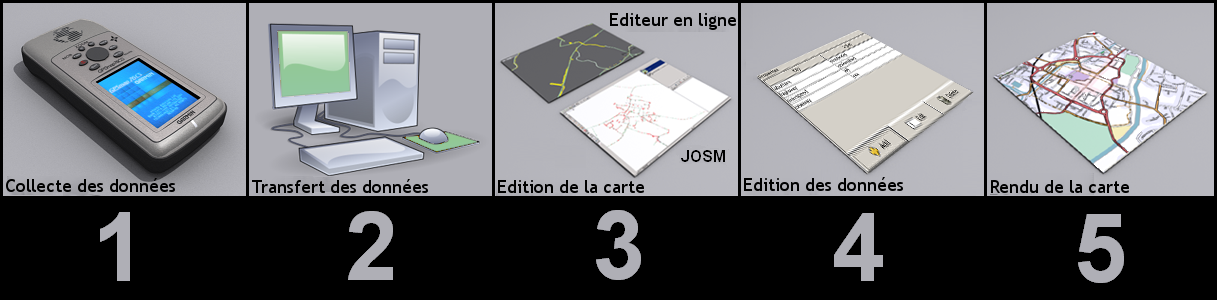
\includegraphics[width=\textwidth]{figures/OSM-steps}

  \begin{enumerate}
  \item Collecter les données
  \item Transférer les données GPS
  \item Générer et éditer les données OSM
  \item Ajouter des labels et des méta-data
  \item Rendu
  \end{enumerate}
}


\frame { \hfill 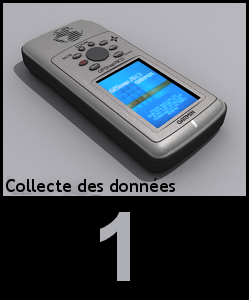
\includegraphics[width=2cm]{figures/OSM-step1}

  Sources de données:
  \begin{itemize}
  \item logs GPS crées par des personnes à pied, à vélo,
      en voiture ou train, qui prennent des notes et photos du trajet
  \item Cadastre numérique (en France)
  \item photos satellite Yahoo! (dans les zones couvertes)
  \item CORINE land cover (en Europe)
  \item imagerie satellite Landsat 7
  \item TIGER (aux USA)
  \item AND (Pays Bas, Chine, Inde)
  \end{itemize}

  \bigskip
  {\large \color{red}\Stopsign{}} Interdiction d'utiliser les cartes propriétaires!
}


\frame { \hfill 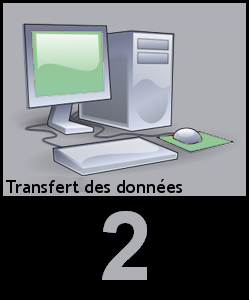
\includegraphics[width=2cm]{figures/OSM-step2}

  \begin{itemize}
  \item Transférer les données vers l'ordinateur
  \item Conversion au format GPX et suppression points redondants
    \begin{itemize}
    \item outil: GPSBabel
    \end{itemize}
  \item Upload des tracks vers OSM via le site web
    \begin{itemize}
    \item nécessite un login
    \end{itemize}
  \end{itemize}
}


\frame { \hfill 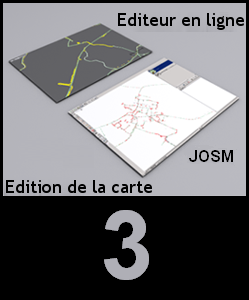
\includegraphics[width=2cm]{figures/OSM-step3}

  \begin{itemize}
  \item Générer et éditer les n\oe{}uds et ways dans OSM
  \item Édition en ligne avec Potlatch (application Flash)
  \item Édition hors-ligne avec JOSM (application Java)
  \item Autres logiciels et scripts d'édition
    \begin{itemize}
    \item import massif de données (ex: Corine)
    \end{itemize}
  \item API REST permettant de développer d'autres applications
  \end{itemize}
}

\frame { \hfill 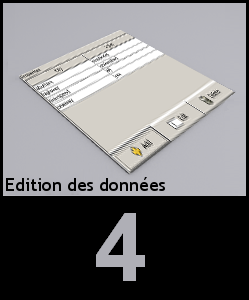
\includegraphics[width=2cm]{figures/OSM-step4}

  \begin{itemize}
  \item Ajouter des étiquettes et méta-données
  \item Ajouter des données aux n\oe{}uds et ways pour permettre leur rendu
  \item Outils d'édition: JOSM, Potlatch
  \item Outils de détection d'incohérences:
    \begin{itemize}
    \item plugin <<~validator~>> pour JOSM
    \item couche <<~maplint~>> des cartes
    \item outils en ligne comme Keepright!, Osmose
    \end{itemize}
  \end{itemize}
}


\frame { \hfill 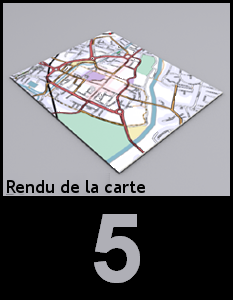
\includegraphics[width=2cm]{figures/OSM-step5}

  \begin{itemize}
  \item Se fait automatiquement une fois que les données sont transférées
    vers le serveur

  \item Application Mapnik
    \begin{itemize}
    \item pré-traitement avec PostGIS pour accélérer le rendu
    \item rendu mis à jour en quelques heures
    \end{itemize}

  \item Application Osmarender (pipeline XSLT)
    \begin{itemize}
    \item possiblité d'utiliser des feuilles de styles XSLT personnalisées pour
      obtenir des cartes spécialisées
    \item possibilité d'exporter les cartes vers du SVG pour retouche manuelle
    \end{itemize}

  \item Visualisation des tuiles depuis une interface web (Slippymap)
    ou depuis applications spécialisées comme Viking
  \end{itemize}
}

\frame { \hfill 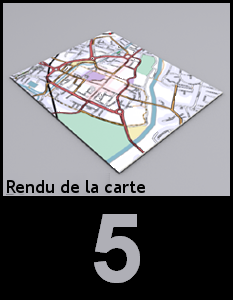
\includegraphics[width=2cm]{figures/OSM-step5}

  %% http://wiki.openstreetmap.org/wiki/List_of_OSM_based_Services
  Plusieurs jeux de tuiles spécialisés existent:
  \begin{itemize}
  \item \href{http://www.opencyclemap.org/}{OpenCycleMap.org}, pistes cyclables, avec topographie
  \item \href{http://www.openpistemap.org/}{OpenPisteMap.org}, carte des pistes
  \item \href{http://www.öpnvkarte.de/}{öpnvkarte.de}, transports en commun
  \item \href{http://www.openseamap.org/}{OpenSeaMap.org}, navigation en mer
  \item \href{http://www.osm-wms.de/}{WMS OSM}, services de mesurage 
  \end{itemize}
}



\frame{\vfill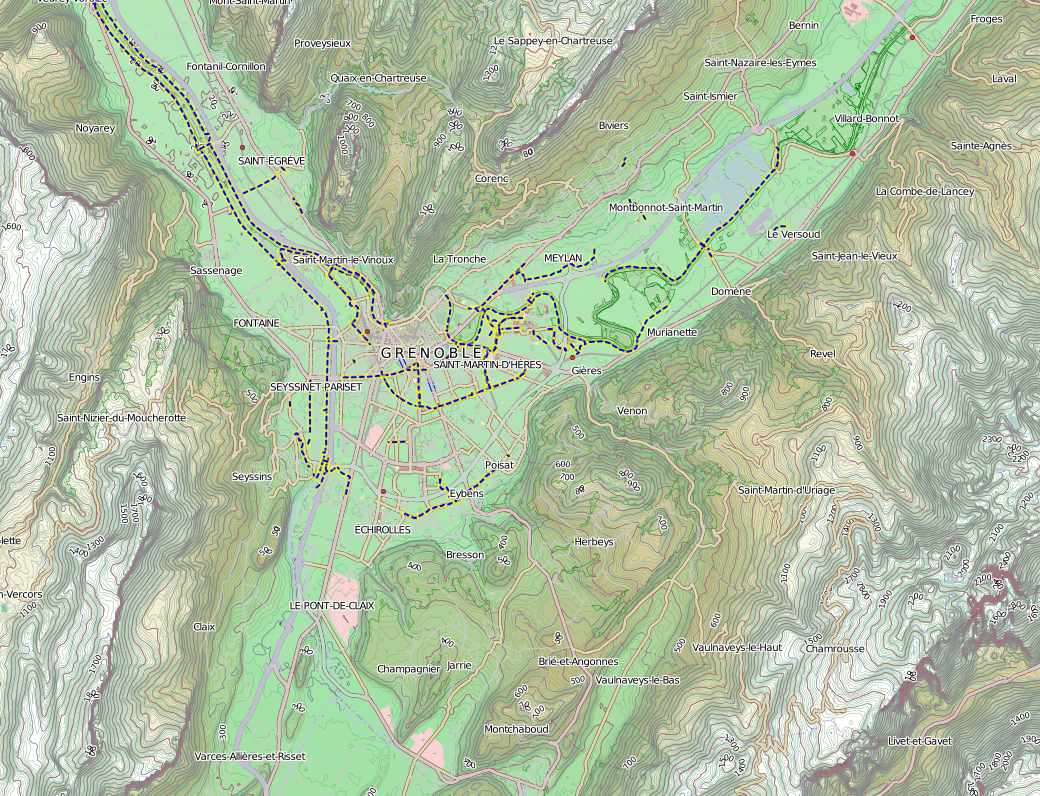
\includegraphics[width=0.95\textwidth]{figures/open-cycle-map}}
\frame{\vfill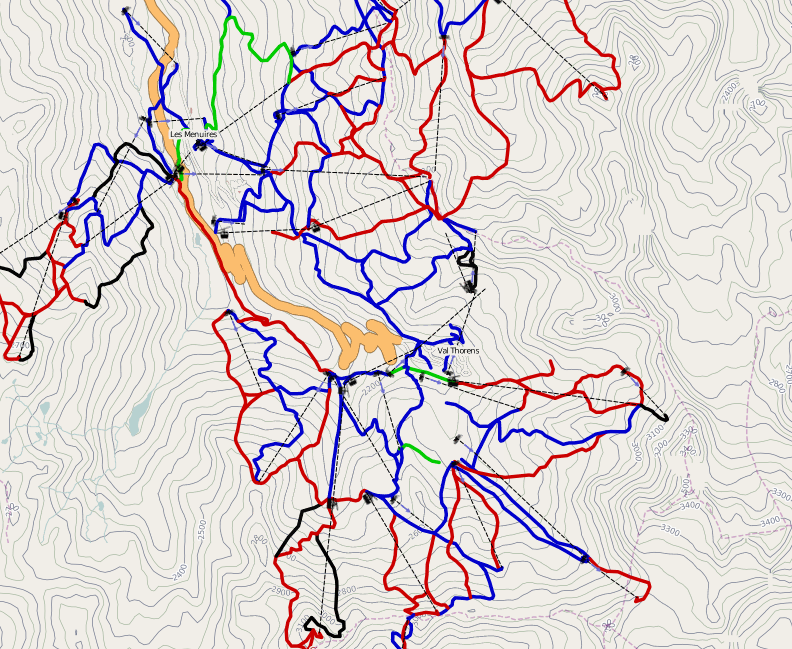
\includegraphics[height=0.94\textheight]{figures/open-piste-map}}
\frame{\vfill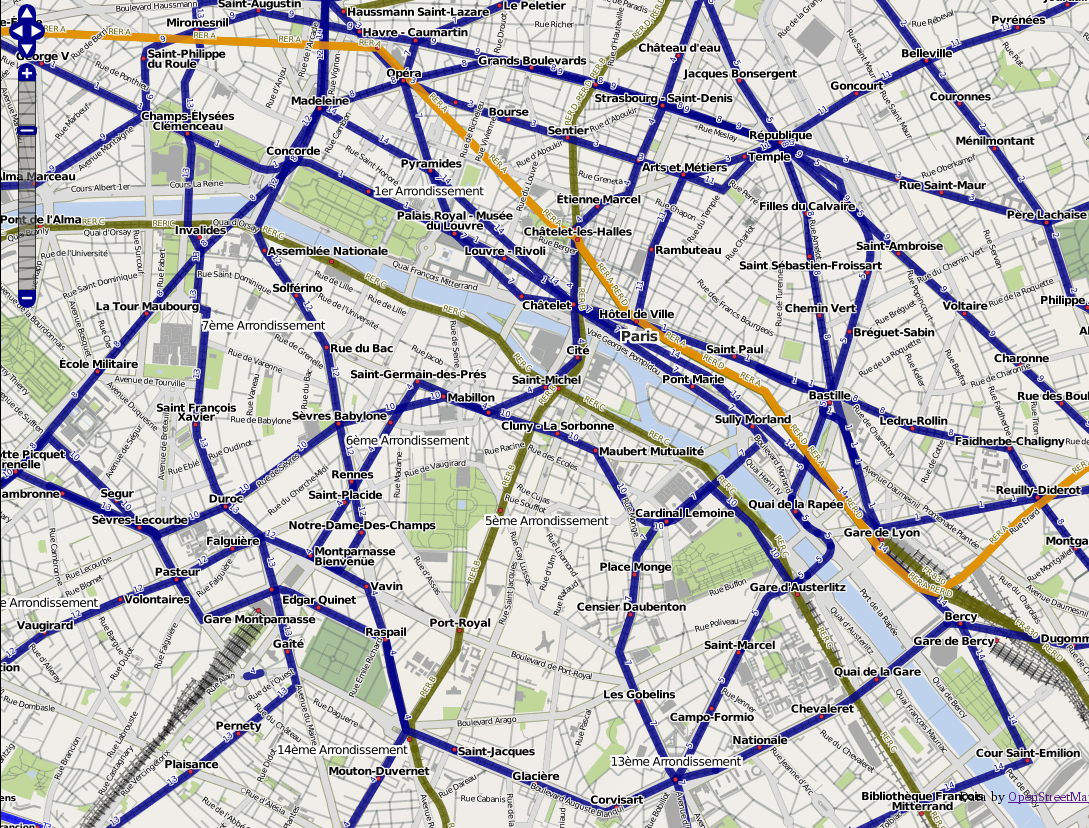
\includegraphics[width=0.95\textwidth]{figures/opnvkarte}}
\frame{\vfill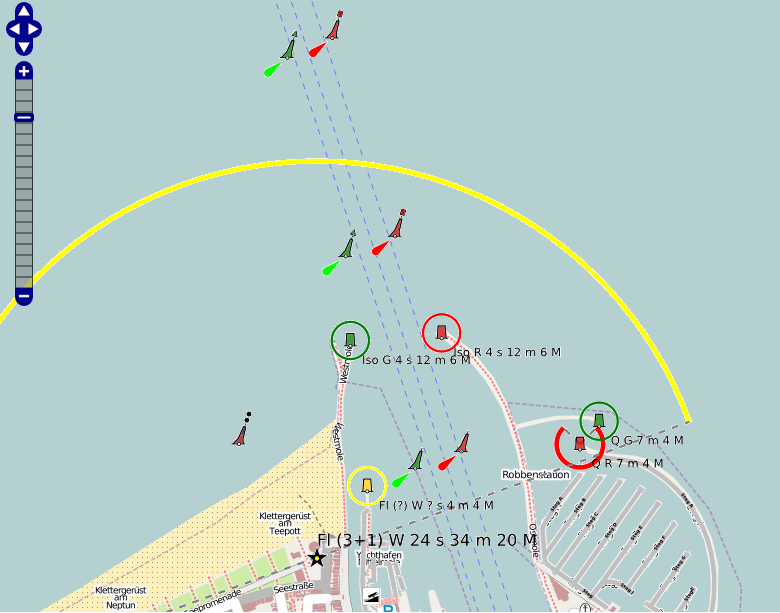
\includegraphics[width=0.95\textwidth]{figures/open-sea-map}}
\frame{\vfill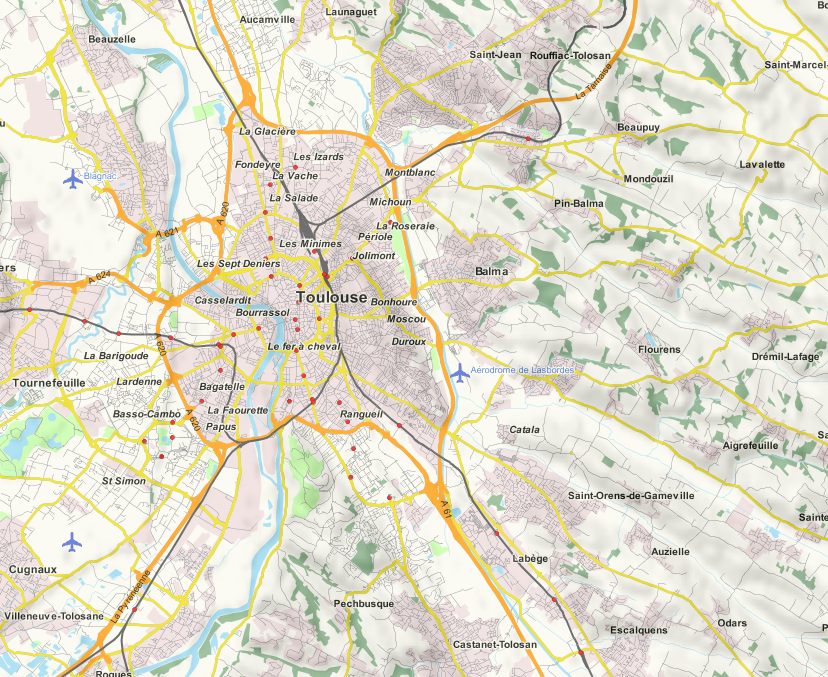
\includegraphics[width=0.95\textwidth]{figures/OSM-WMS}}
\frame{\vfill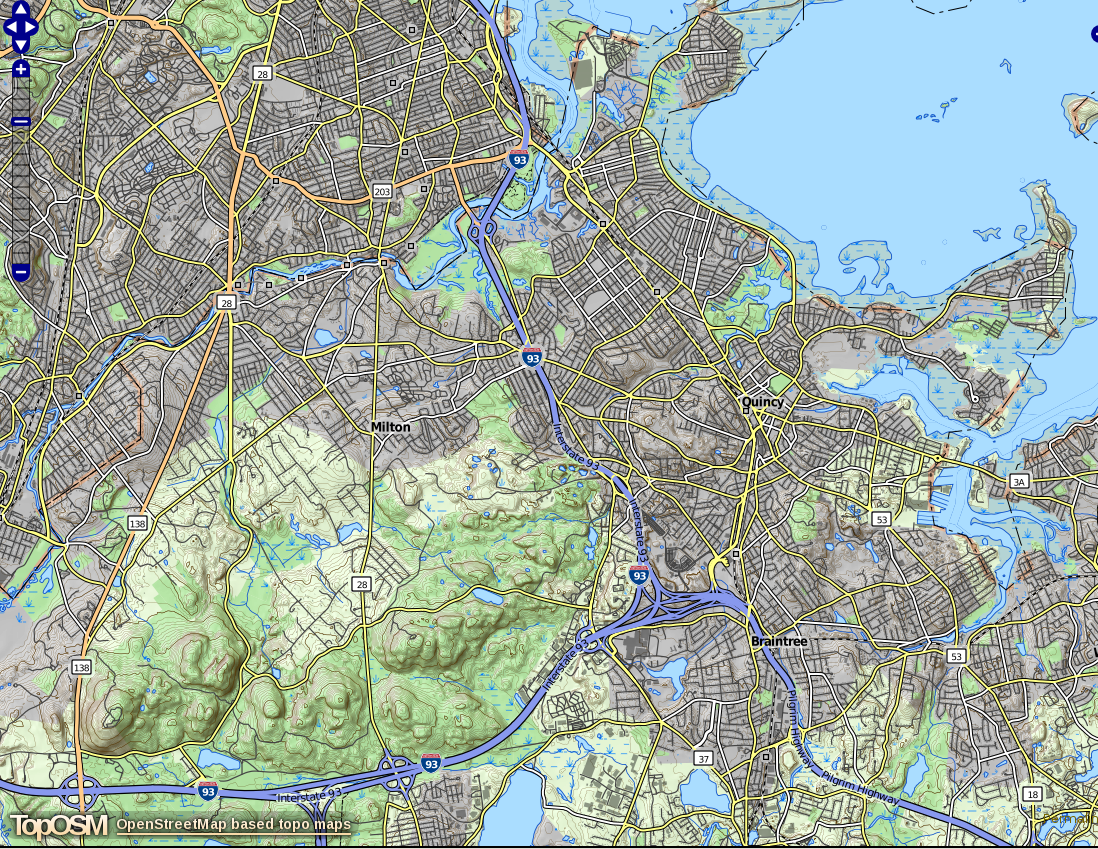
\includegraphics[width=0.95\textwidth]{figures/toposm}}




\frame{ \heading{Structuration technique} \vfill

Structures de données employées:
\begin{itemize}
\item Un \textit{n\oe{}ud} est un point représentant une position
\item Un \textit{way} (ou chemin) est une séquence de n\oe{}uds,
  représentant une polyligne ou un polygône
\item Une \textit{relation} est un ensemble de n\oe{}uds et de ways
  auxquels on donne des propriétés 
\item Une \textit{étiquette} ou tag peut être appliquée à un n\oe{}ud, un
  way ou une relation, et consiste de paires \texttt{nom=valeur}
\end{itemize}

\bigskip
La sémantique des étiquettes est \href{http://wiki.openstreetmap.org/index.php/Map_Features}
{décrite sur un wiki}. 
}


% http://wiki.openstreetmap.org/index.php/Map_Features
\frame{ \heading{Étiquettage} \vfill

  Exemples:
  \begin{itemize}
  \item highway = motorway
  \item junction = roundabout
  \item oneway = yes
  \item cycleway = lane
  \item waterway = canal
  \item railway = station
  \item railway = subway
  \item leisure = park
  \item amenity = pub
  \item shop = supermarket
  \item tourism = zoo
  \end{itemize}

}


%% EOF

%% demo.tex
%%
%% Time-stamp: <2009-12-05 emarsden>


\section{Démonstration}

\frame[plain]{  \heading{Plan de la Présentation}
\ecmsetupplan
\begin{itemize}
  \item[\small $\Diamond$] Introduction
  \item[\small $\Diamond$] Fonctionnement
  \item[\small $\Diamond$] {\color{purple}\textbf{Démonstration}}
  \item[\small $\Diamond$] Applications
  \item[\small $\Diamond$] Conclusions
\end{itemize}
}


\frame{ \heading{Démo: créer une carte personnalisée}  \vfill
  \begin{minipage}{0.45\textwidth}
    \begin{enumerate}
    \item Trouver la zone pertinente dans le slippymap
    \item Ouvrir le tab ``Export''
    \item Sélectionner le format (PDF, SVG, PNG, XML)
    \item Exporter
    \item Éditer le SVG dans Inkscape
    \end{enumerate}
  \end{minipage} \quad %
  \begin{minipage}{0.49\textwidth}
    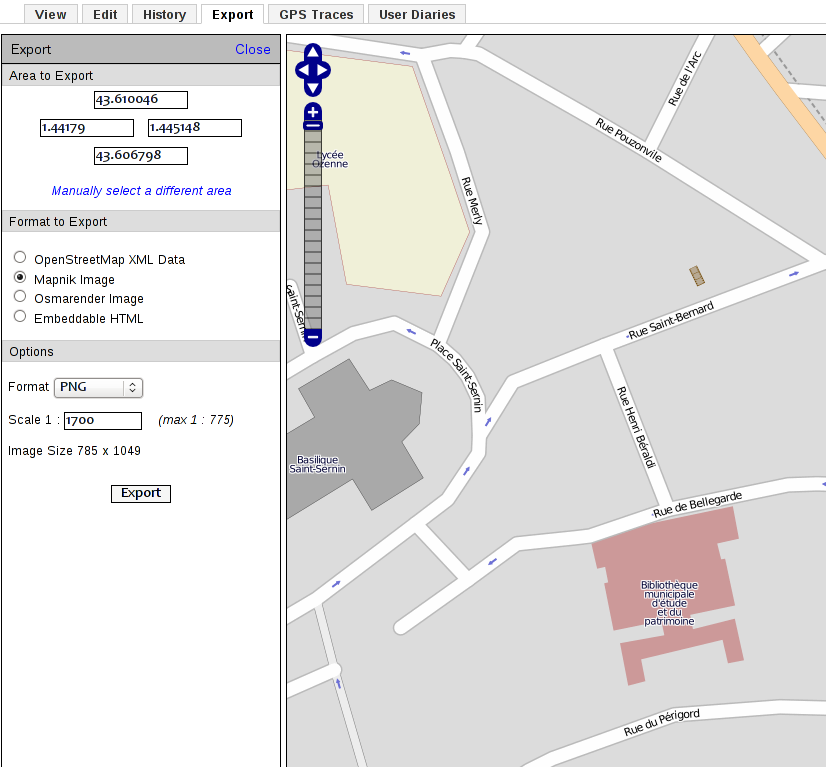
\includegraphics[width=\textwidth]{figures/OSM-export}
  \end{minipage}
}



\frame{ \heading{Démo: corriger un nom de rue}  \vfill
  \begin{minipage}{0.45\textwidth}
    \begin{enumerate}
    \item Trouver la rue dans le slippymap
    \item Ouvrir le tab ``Edit''
    \item S'identifier
    \item Sélectionner la voie
    \item Changer le nom
    \end{enumerate}
  \end{minipage} \quad %
  \begin{minipage}{0.49\textwidth}
    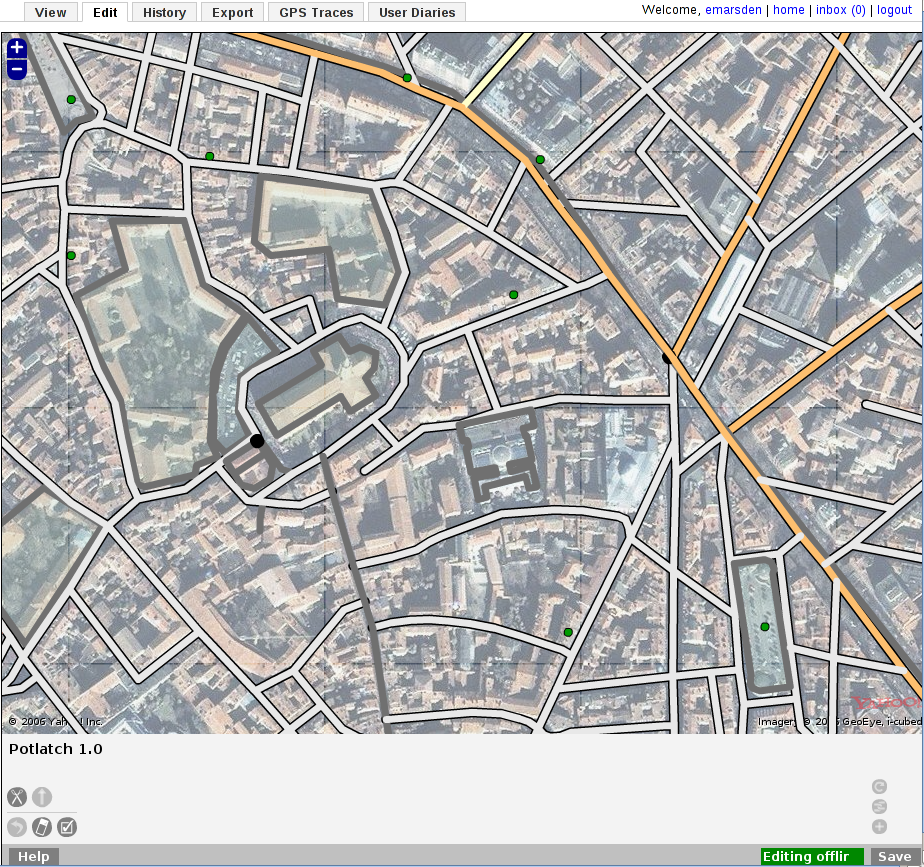
\includegraphics[width=\textwidth]{figures/potlatch}
  \end{minipage}
}


\frame{ \heading{Démo: ajouter une voie cyclable}  \vfill
  \begin{minipage}{0.45\textwidth}
    \begin{enumerate}
    \item Ouvrir JOSM
    \item Télécharger la zone pertinente
    \item Sélectionner la voie
    \item Découper le tronçon pertinent
    \item Ajouter tag \texttt{cycleway=left}
    \end{enumerate}
    \end{minipage} \quad %
  \begin{minipage}{0.49\textwidth}
    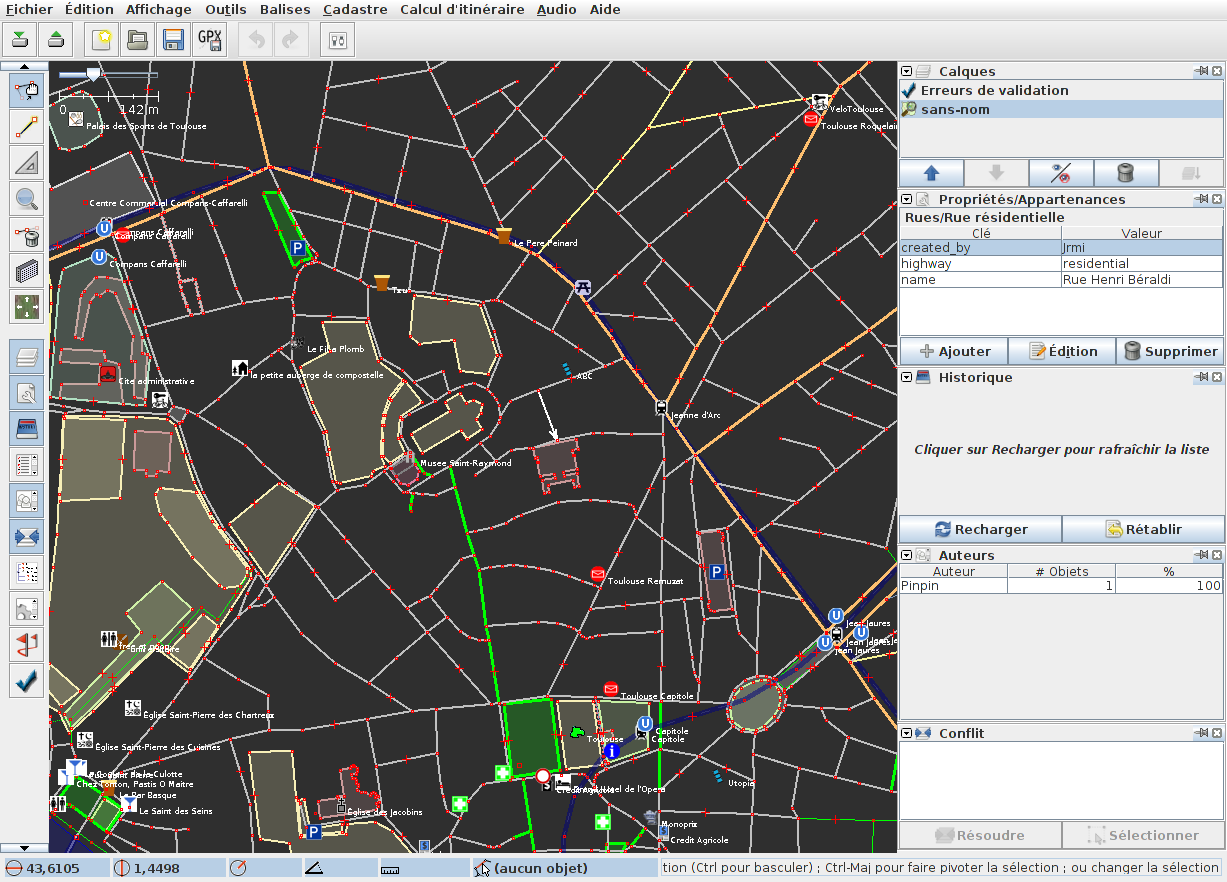
\includegraphics[width=\textwidth]{figures/JOSM}
  \end{minipage}
}

\frame{ \heading{Démo: ajouter son bar favori}  \vfill
\begin{enumerate}
\item Ouvrir JOSM et télécharger la zone pertinente
\item Récupérer une vue cadastre de la zone (ou waypoint GPS)
\item Créer un n\oe{}ud au bon endroit
\item Ajouter des tags \texttt{amenity=bar} (ou \texttt{pub} ou \texttt{nightclub})
\item Préciser le nom du bar en ajoutant un tag \texttt{name=La Tireuse}
\item Uploader les données
\end{enumerate}
}

\frame{ \heading{Démo: tracer une nouvelle route depuis un gpx}  \vfill
\begin{enumerate}
\item Néttoyer le fichier gpx de points inutiles
\item Ouvrir le tab ``GPS Traces''
\item S'identifier
\item Uploader son fichier gpx
\item Télécharger la zone dans JOSM
\item Tracer depuis la couche gpx
\end{enumerate}
}

\frame{ \heading{Démo: Lakewalker pour tracer un lake}  \vfill
\begin{enumerate}
\item Installer les plugins lakewalker \& WMS
\item Naviguer vers une zone avec un lac
\item Récupérer un fond Landsat pour la zone
\item Activer le plugin lakewalker
\item Vérifier les données
\item Uploader les changements
\end{enumerate}
}



%% new typographic/map explosion
%% http://calebwaldorf.net/reblog/typologies-from-the-new-cartographic-explosion/



%% EOF

%% osm-applications.tex
%%


\section{Applications}

\frame[plain]{  \heading{Plan de la Présentation}
\ecmsetupplan
\begin{itemize}
  \item[\small $\Diamond$] Introduction
  \item[\small $\Diamond$] Fonctionnement
  \item[\small $\Diamond$] {\color{purple}\textbf{Applications}}
  \item[\small $\Diamond$] Conclusions
\end{itemize}
}



%% http://www.foss4g2007.org/presentations/view.php?abstract_id=56


\frame { \heading{Utilisations des données} \vfil

  %% http://wiki.openstreetmap.org/index.php/Fr:Using_OpenStreetMap
  
  %% http://fredericbonifas.free.fr/osm.html

  %% http://wiki.navit-project.org/images/thumb/f/fa/FBZH-gtk.png/800px-FBZH-gtk.png
  
  \begin{minipage}{0.8\textwidth}
  \begin{itemize}
  \item guidage temps réel (applications: pyroute, navit, GPSDrive,
    gosmore, roadnav) 
  \item cartes et applications de routage thématiques
    \begin{itemize}
    \item spécifique vélo ou piéton ou bâteau
    \item carte des châteaux d'une zone viticole
    \item préparation d'un \textit{pub crawl}
    \end{itemize}
  \item utiliser les données dans des simulateurs
    \begin{itemize}
    \item existe pour FlightGear (avec terragear)
    \item idée Guilhem: simulateur de conduite automobile
    \end{itemize}
  \item permet un réalisme troublant
    \begin{itemize}
    \item localisations des boîtes aux lettres, points de recyclage,
      toilettes, bornes SOS
    \end{itemize}
  \item insérer votre idée ici: les données sont libres!
  \end{itemize}
  \end{minipage} %
  \begin{minipage}{0.19\textwidth}
    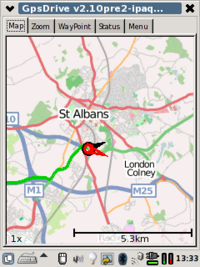
\includegraphics[width=1.5cm]{figures/200px-Gpsdrive_ipaq_screenshot-map-z11}
    \vskip 1cm

    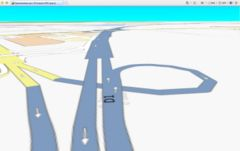
\includegraphics[width=1.5cm]{figures/240px-Now_turn_right2}
    \vskip 1cm
    
    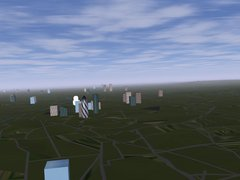
\includegraphics[width=1.5cm]{figures/240px-Osmroads1}
    \vskip 1cm
  \end{minipage}
}

\frame{ \heading{Utilisation sur terminal mobile} \vfil
  \begin{tikzpicture}[remember picture,overlay,font={\footnotesize},text
    width=2cm,text centered]
   \node[xshift=1cm,yshift=-4cm] at (current page.north west) {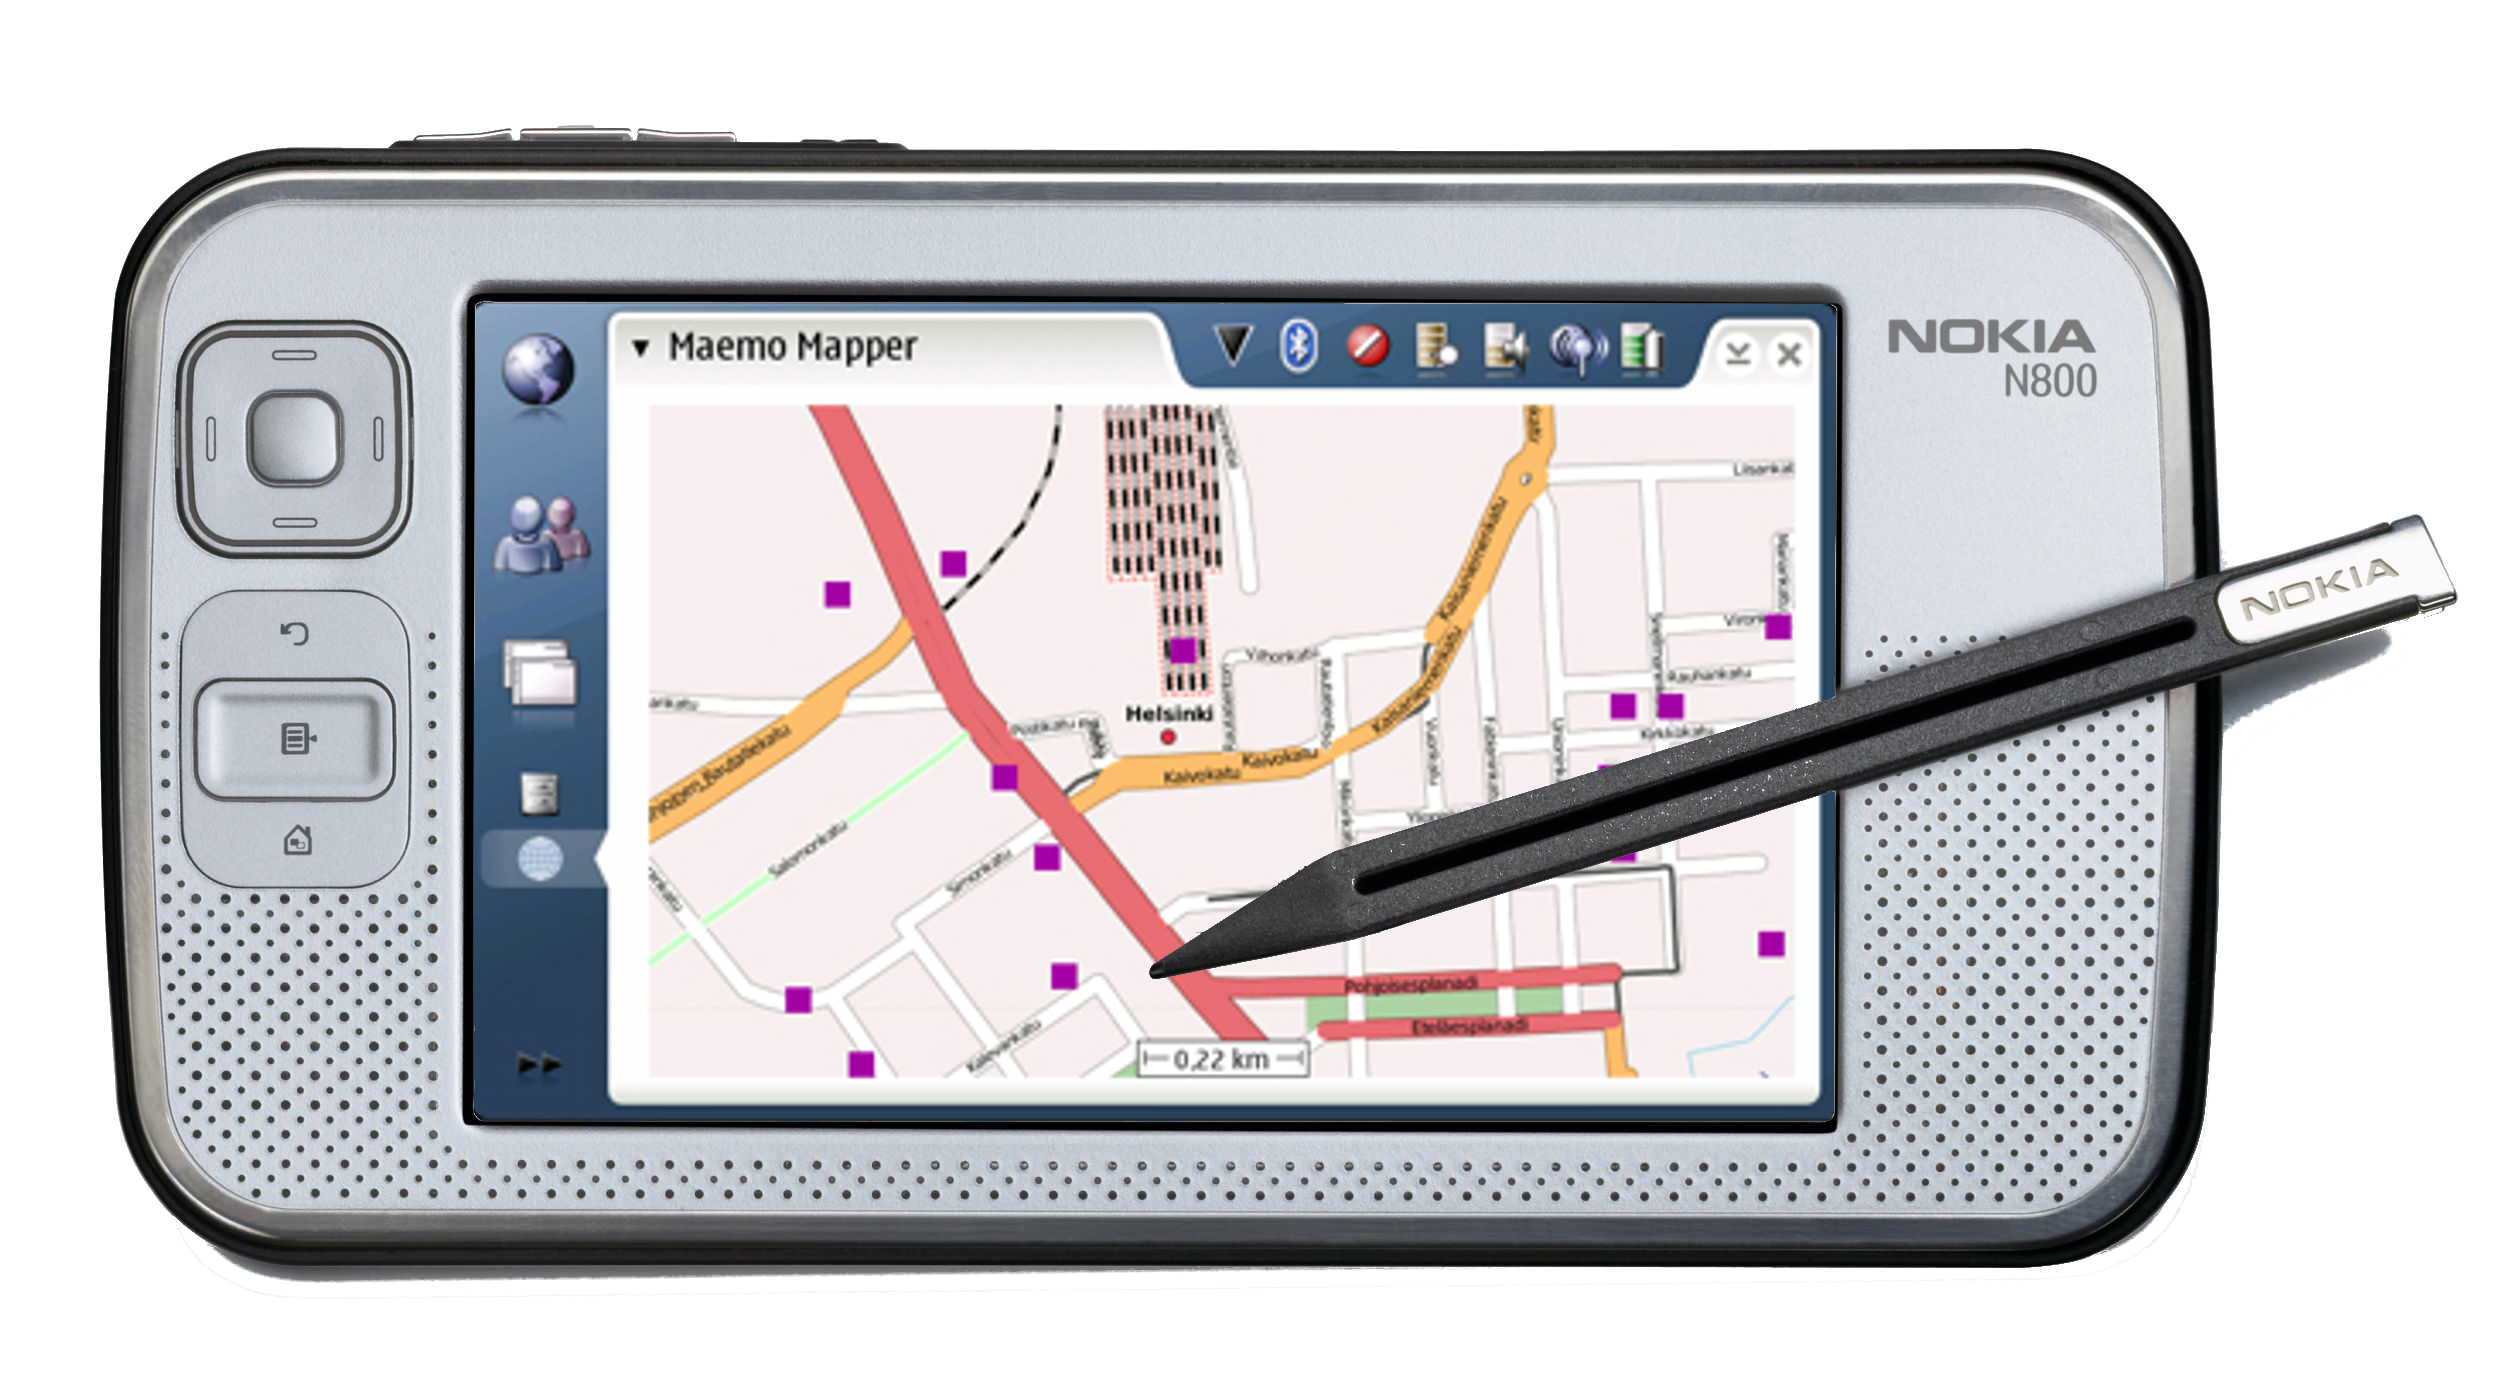
\includegraphics[width=7cm]{figures/osm-N800}};
   \node[xshift=-1cm,yshift=-3cm] at (current page.north east) {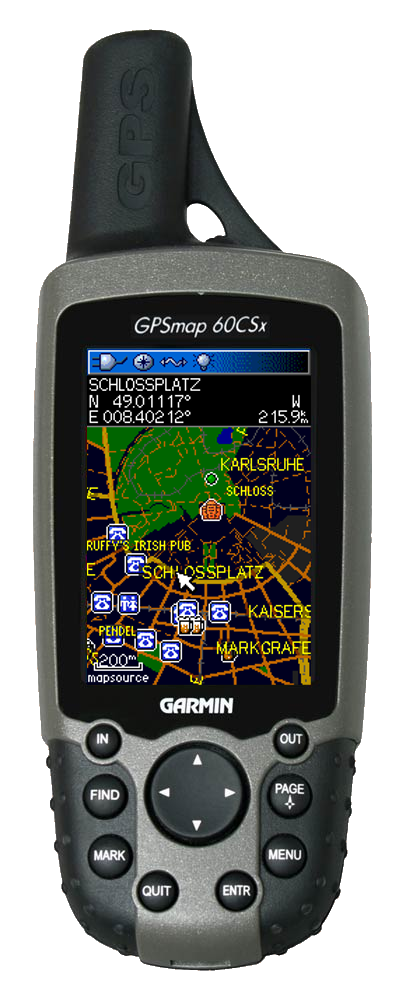
\includegraphics[height=5cm]{figures/OSM-garmin}};
   \node[xshift=-4.7cm,yshift=3.5cm] at (current page.south east) {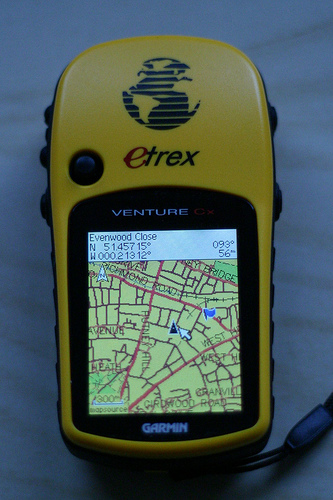
\includegraphics[height=5cm]{figures/OSM-garmin-etrex}};
\end{tikzpicture}
}


%% http://www.geographie.uni-bonn.de/karto/osm-3d/screenshots.en.htm

%% EOF

%% osm-conclusions.tex
%%


\section{Conclusions}

\frame{ \heading{Perspectives} \vfill

  \begin{itemize}
  \item processus de revue, alerte email en cas de modif zone reviewé
  \item services de «données néttoyées» pour utilisations critiques
    \begin{itemize}
    \item validation de la qualité des ajouts/suppressions de données
    \item homogénisation des tags
    \end{itemize}
    
  \item meilleure gestion des rollback en cas d'erreur volontaire ou malveillant

  \item[{\color{darkyellow}\Lightning}] outils pour gérer un «édit war»:
    \begin{itemize}
    \item prévention: permettre des rendus par langue
    \item locks par objet/zone géographique contestée 
    \item désignation de modérateurs
    \end{itemize}
  \item éventuel changement de licence: CCBYSA $\rightarrow$ ``Open Database Licence''
  \end{itemize}
}



\frame{ \heading{Conclusions} \vfill

  Intérêts des cartes libres:
  \begin{itemize}
  \item utilisation libre des données cartographiques
    \begin{itemize}
    \item créer un logiciel de navigation libre
    \item créer des cartes spécifiques liés à ses propres intérêts
    \item illustrer des documents libres
    \end{itemize}

  \item permettre de corriger des erreurs dans les cartes (rues
    devenues en sens unique, \ldots{})
  \end{itemize}

  \bigskip
  
  Limites:
  \begin{itemize}
  \item couverture encore très inférieure aux solutions propriétaires en France
  \item qualité des données non garantie (vandalisme, \ldots{})
  \end{itemize}

}


% Convention d'Aarhus
%   Signée le 15 juin 1998 ratifiée en France par la
%   loi du 28 février 2002 et du 26 octobre 2005
% • les trois piliers de la Convention
%    – développer l’accès du public à l’information détenue
%      par les autorités publiques,
%    – favoriser la participation du public à la prise des
%      décisions liées à l’environnement,
%    – étendre les conditions d’accès à la justice.



\frame{ \heading{Pour en savoir plus} \vfill

  \begin{itemize}
  \item Site web: \url{http://openstreetmap.org/}
  \item Courriel: \url{talk-fr@openstreetmap.org}
  \item IRC: \#osm-fr sur le serveur \texttt{irc.oftc.net}
  \item Animations de l'évolution du projet: \url{http://www.jabberworld.org/osm/}
  \end{itemize}


  \vfill

  \begin{beamerboxesrounded}[width=\textwidth,scheme=alert,shadow=true]{} \sffamily\tiny
  Cette présentation est diffusable selon les termes de la license
  CC-BY-SA 2.0. Des éléments ont été repris de présentations préparées
  par:
  \begin{itemize}
  \item Émmanuel Garette
  \item Frederik Ramm
  \item Jochen Topf
  \item Sylvain Beorchia \& Thomas Walraet
  \end{itemize}

  \end{beamerboxesrounded}

}


%% EOF

\end{document}

%% EOF
